\documentclass[letterpaper,10pt]{article}

\usepackage{titling}
\usepackage{listings}
\usepackage{url}
\usepackage{setspace}
\usepackage{subfig}
\usepackage{sectsty}
\usepackage{pdfpages}
\usepackage{colortbl}
\usepackage{multirow}
\usepackage{multicol}
\usepackage{relsize}
\usepackage{amsmath}
\usepackage{wasysym}
\usepackage{fancyvrb}
\usepackage{amsmath,amssymb,amsthm,graphicx,xspace}
\usepackage[titlenotnumbered,noend,noline]{algorithm2e}
\usepackage[compact]{titlesec}
\usepackage{XCharter}
\usepackage[T1]{fontenc}
\usepackage{tikz}
\usetikzlibrary{arrows,automata,shapes,trees,matrix,chains,scopes,positioning,calc}
\tikzstyle{block} = [rectangle, draw, fill=blue!20, 
    text width=2.5em, text centered, rounded corners, minimum height=2em]
\tikzstyle{bw} = [rectangle, draw, fill=blue!20, 
    text width=4em, text centered, rounded corners, minimum height=2em]

\definecolor{namerow}{cmyk}{.40,.40,.40,.40}
\definecolor{namecol}{cmyk}{.40,.40,.40,.40}

\let\LaTeXtitle\title
\renewcommand{\title}[1]{\LaTeXtitle{\textsf{#1}}}


\newcommand{\handout}[5]{
  \noindent
  \begin{center}
  \framebox{
    \vbox{
      \hbox to 5.78in { {\bf ECE459: Programming for Performance } \hfill #2 }
      \vspace{4mm}
      \hbox to 5.78in { {\Large \hfill #4  \hfill} }
      \vspace{2mm}
      \hbox to 5.78in { {\em #3 \hfill} }
    }
  }
  \end{center}
  \vspace*{4mm}
}

\newcommand{\lecture}[3]{\handout{#1}{#2}{#3}{Lecture #1}}
\newcommand{\tuple}[1]{\ensuremath{\left\langle #1 \right\rangle}\xspace}

\addtolength{\oddsidemargin}{-1.000in}
\addtolength{\evensidemargin}{-0.500in}
\addtolength{\textwidth}{2.0in}
\addtolength{\topmargin}{-1.000in}
\addtolength{\textheight}{1.75in}
\addtolength{\parskip}{\baselineskip}
\setlength{\parindent}{0in}
\renewcommand{\baselinestretch}{1.5}
\newcommand{\term}{Winter 2017}

\singlespace



\begin{document}

\section*{ECE 459 Assignment Setup Guide}

The assignments are designed and tested using the \texttt{ecelinux} and \texttt{ecetesla} servers (connection and setup guide below). Although you can develop and test the code on your own laptop, course staff will only support running on \texttt{ecelinux}/\texttt{ecetesla}, so if you're having problems on your laptop we'll say try it there. 

Preferably in advance of the actual first assignment for the term, you should do the following things:
\begin{itemize}
	\item Set up and configure your \url{git.uwaterloo.ca} account.
	\item Test if you can log in via ssh to \texttt{ecelinux} servers. If you can't, please contact Eric Praetzel, part of the ECE lab staff,  at \texttt{praetzel@uwaterloo.ca} .
\end{itemize}

\subsection*{Starting with Gitlab}
Gitlab is a web-based software product for managing source control repositories. The University of Waterloo runs this as a service at \url{git.uwaterloo.ca}. If you navigate there, you'll be presented with this login screen, where you can log in with your Central Authentication Service credentials (same ones for Quest, etc.). 

\begin{center}
	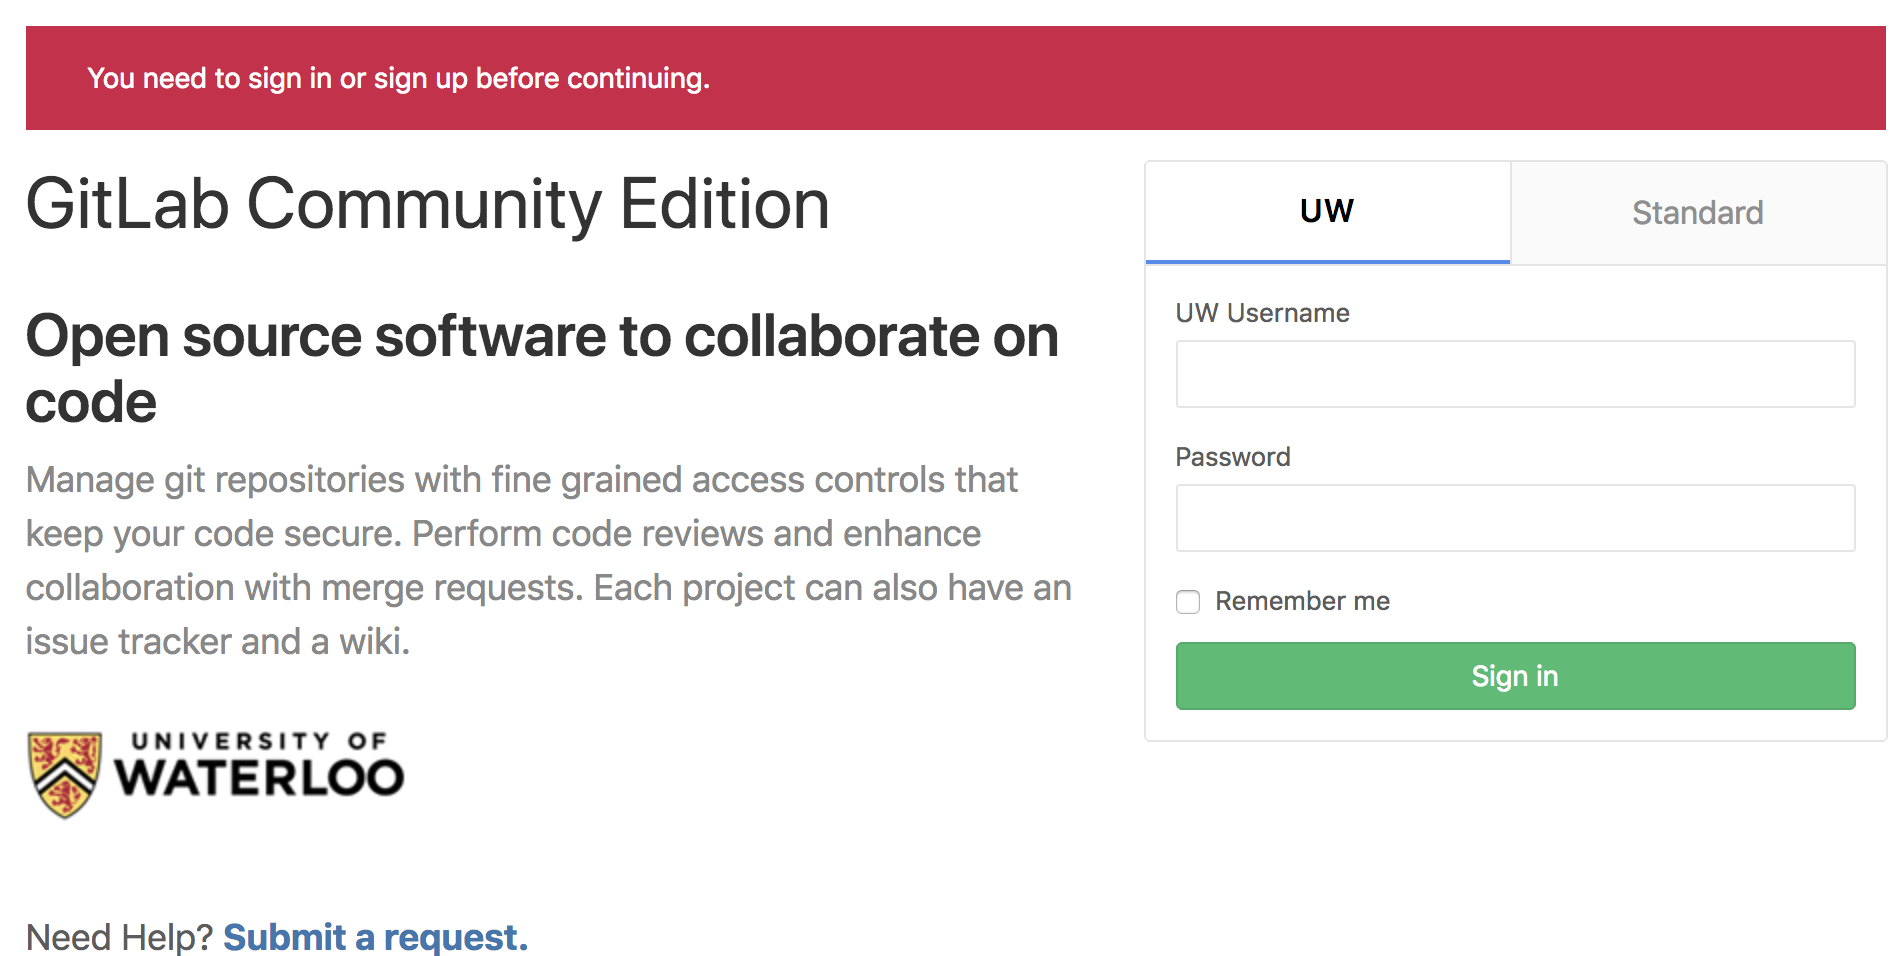
\includegraphics[width=0.6\textwidth]{images/gitlab-login.png}
\end{center}

If you haven't logged in before and haven't set up your account before, then you need to do some one-time setup. If you've done that already, you can skip to the next section.

When logged in, you can set up your profile (to whatever detail you wish). But most importantly you will need to generate an secure shell key. Under ``profile settings'', click on SSH Keys, as shown below. In the image, a red box surrounds the the link you can click on for instructions about how to generate a new SSH Key, or find yours if you already have one. If you have an SSH Key already, you should also put it on \texttt{ecelinux} as well; if you don't then you can generate yours on the server so you don't have to copy it.

\begin{center}
	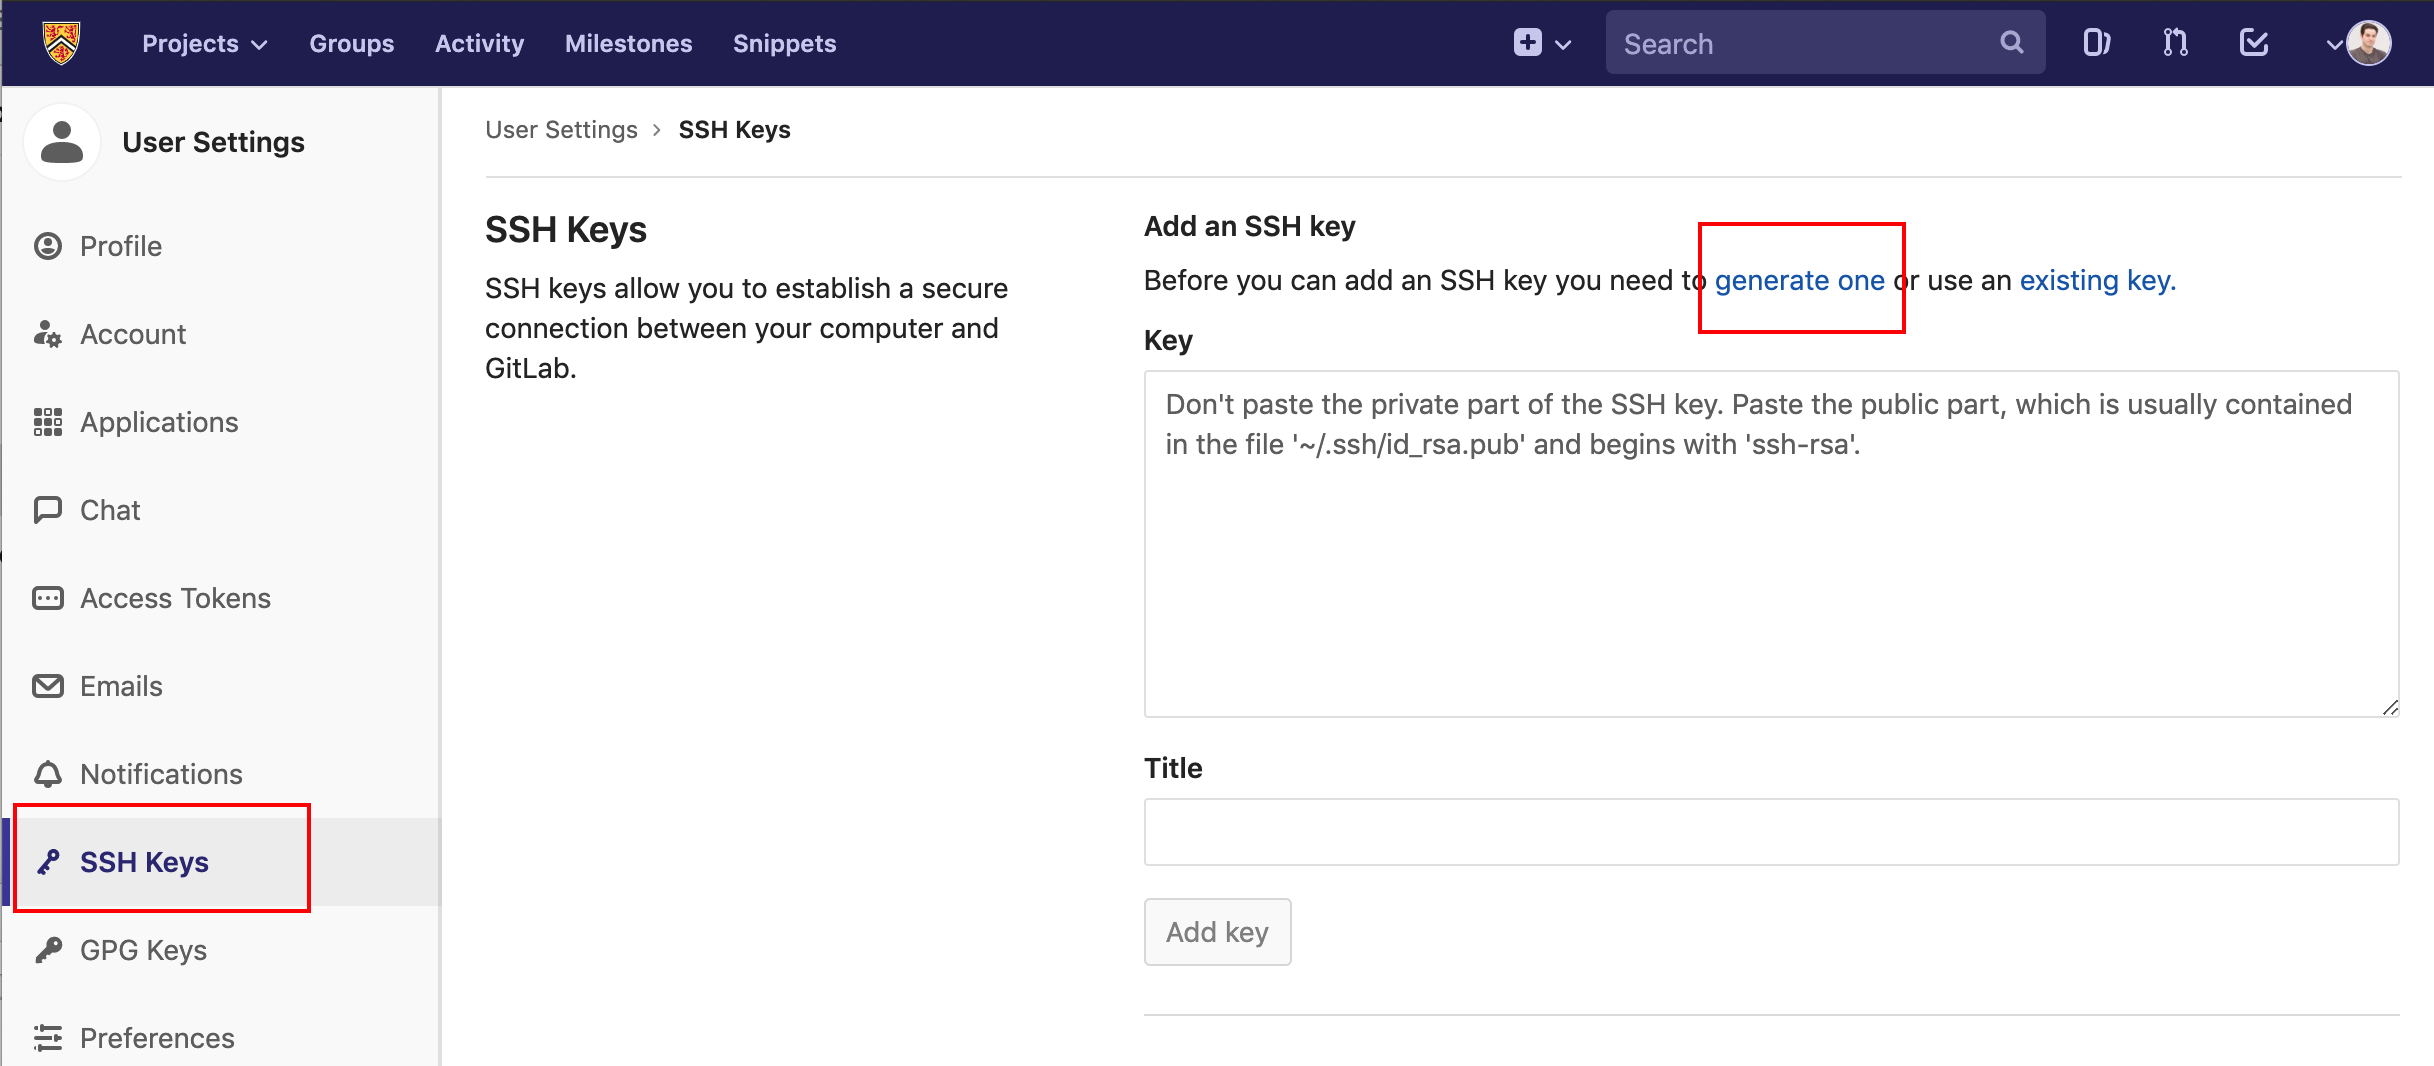
\includegraphics[width=0.9\textwidth]{images/gitlab-sshkey.png}
\end{center}

You need to add this key to your gitlab account so that when you want to interact with the git repository, the key is used to identify you.

\subsection*{Connecting to \texttt{ecelinux}/\texttt{ecetesla}}

The \texttt{ecelinux} name refers to a grouping of servers (\texttt{ecelinux1}, \texttt{ecelinux2},...). The same is true for \texttt{ecetesla}. Although the servers have some hardware differences, they are not usually relevant for the purposes of the assignment. They also share a file system, so any one is as good as any others, and if you find that one server is particularly busy you can move to another one and pick up where you left off. Even if you are not an ECE student, being registered in an ECE course should grant you access to the servers.

Your login credentials (i.e., username and password) are the same as your WatIAM ones. The server full name is \texttt{ecelinux.uwaterloo.ca} or \texttt{ecetesla.uwaterloo.ca} and most of the other options like port, etc. can be left as the defaults. 

If you're using Linux or macOS, open a terminal and connect by typing \texttt{ssh USERID@ecelinux.uwaterloo.ca}, obviously replacing USERID with your actual userid. To connect to these servers, you need to be inside the campus firewall, except \texttt{ecelinux4.uwaterloo.ca}. And then you are connected. 

If you're using Windows 10, you can set up Powershell to be able to use \texttt{ssh} directly. Instructions are at \url{https://www.howtogeek.com/336775/how-to-enable-and-use-windows-10s-built-in-ssh-commands/} . If that's all set up and working then you just connect using the same command as in Linux/macOS.

You can also use a third party client to connect such as PuTTY or MobaXterm or anything else that you like. For space reasons I won't repeat exactly how to configure them, but they are relatively self-explanatory. You can use any client you want to connect; just read the documentation of it for how to get started.

If you want to transfer files between your local machine and the ECE department servers you can use a SFTP (SSH File Transfer Protocol, or Secure File Transfer Protocol) client. If you do the whole assignment on \texttt{ecelinux}/\texttt{ecetesla} then you don't have to move files.

If you have everything set up correctly, when you log in you will be presented with a little login message (news and updates and information from the lab staff, which you should read) and be presented with the command prompt. Ready to go!

\subsection*{Use of \texttt{git}}
If you would like to learn more about \texttt{git} or are just interested in the full reference you can use \url{https://git-scm.com/book/en/v1/Getting-Started} (or just search the particular command you would like to use). The commands shown here are the absolute bare minimum you need to know for a scenario where (1) you've never used \texttt{git} before, and (2) you work only on \texttt{ecelinux}/\texttt{ecetesla} and don't incorporate changes from anywhere else or any other users.

If you haven't used git before, you need to set your name and email. So use these commands, obviously replacing FIRSTNAME, LASTNAME, and USERID with the actual values. 
\begin{lstlisting}
git config --global user.name "FIRSTNAME LASTNAME"
git config --global user.email "USERID@edu.uwaterloo.ca"
\end{lstlisting}

When checking out a repository for the first time, use \texttt{git clone}, which takes as an argument the URL of the repository to clone. The URL for your repository is found in gitlab:

\begin{center}
	
\includegraphics[width=0.9\textwidth]{images/gitlab-clone.png}
\end{center}

Copy the value from the highlighted box. It takes a moment to clone the repository. If it's not going well, make sure you have your ssh key set up. 

Then you're ready to start working on the code. When you have made some changes you can add those changes to a ``commit'' using the command \texttt{git add}, such as \texttt{git add example.c}. To actually save those changes to your local repository, use the command \texttt{git commit}. This will tell you which files are being committed, and ask you for a commit message. You should write some meaningful message describing the work done.

You need to send any commits you have made back to gitlab using \texttt{git push}. Make sure your commits include all changes that you want to submit; if you've modified files since your last commit those changes do not get pushed unless they are part of a commit. You can push as many times as you like.

You can verify your changes were successfully pushed using the \url{git.uwaterloo.ca} web UI. Check to make sure the files you've changed are up to date there. The course staff sees what is in gitlab so make sure it's correct!

\end{document}
